\begin{frame}{DISTILLED-SINGLE-SHOT-DETECTOR (DSSD)}
    {\bfseries{\scriptsize{(Steps 5 e 6)}}}
    \vspace{-1.8cm}
    \begin{figure}
        \centering
        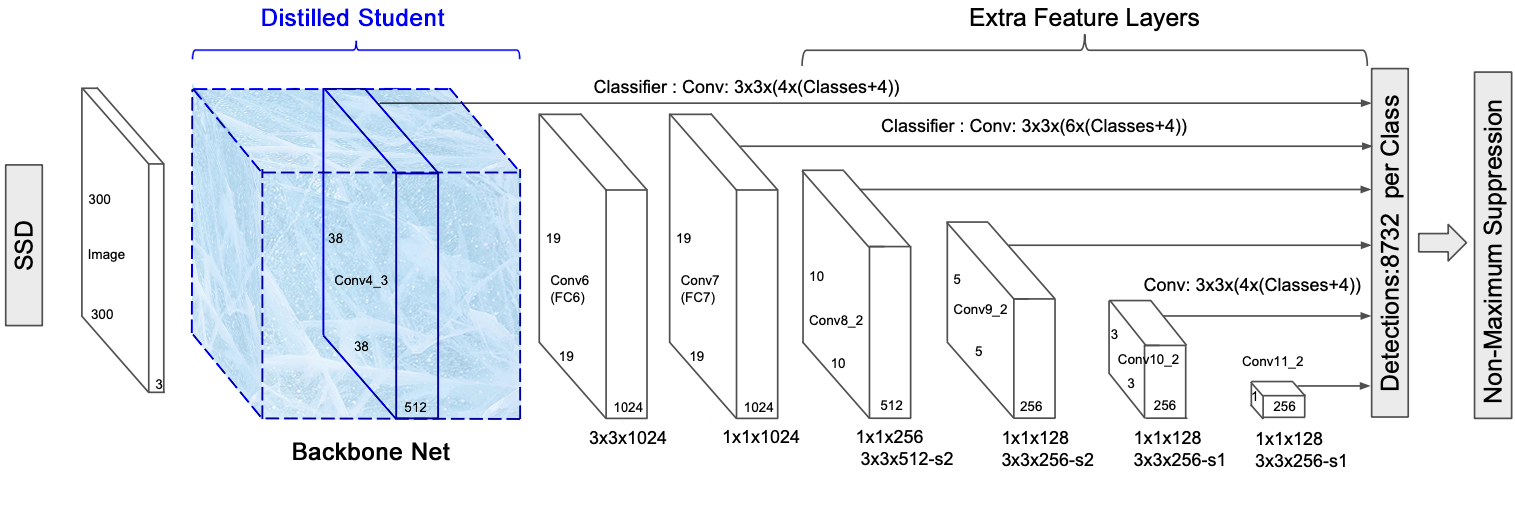
\includegraphics[width = \linewidth]{SSD_architecture_freeze.png}
        \centering
    \end{figure}
    \vspace{-0.5cm}
    \begin{minipage}{\linewidth}
        \centering
        \begin{minipage}{0.40\linewidth}
            {\footnotesize
                \vspace{-0.3cm}
                \begin{block}{\centering 5. Integrazione}
                    Studente distillato come rete "{\bfseries{\emph{backbone}}}" nell'architettura {Single-Shot-Detector (SSD)}.    
                \end{block}
                \vspace{-0.2cm}
                \begin{block}{\centering 6. Training Freeze}
                    Training (\emph{from scratch}) del modello DSSD {\bfseries{\emph{"congelando"}}} la rete \emph{backbone}.
                \end{block}
            }%
        \end{minipage}
        %\hspace{0.5cm}
        \begin{minipage}{0.55\linewidth}
            \begin{figure}
                \centering
                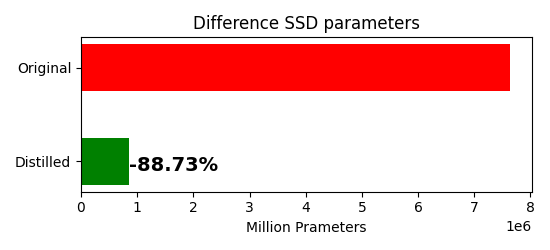
\includegraphics[width = 0.8\linewidth]{Difference SSD parameters.png}
                \centering
            \end{figure}
            \vspace{-0.7cm}
            \begin{figure}
                \centering
                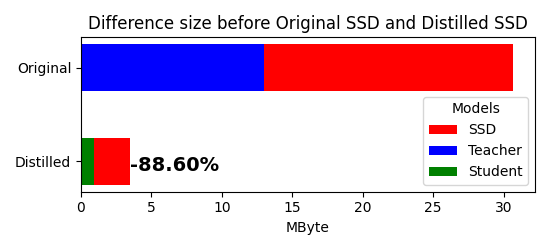
\includegraphics[width = 0.8\linewidth]{Different size SSD.png}
                \centering
            \end{figure}
        \end{minipage}
        \vspace{-2.5cm}
        %{\vspace{-2.5cm}\hspace{-1cm}\reflectbox{\rotatebox[origin=c]{90}{\fontsize{18mm}{19mm}\selectfont{$\curvearrowleft$}}}}
    \end{minipage}   
    \begin{textblock}{10}(109,65)
        \reflectbox{\rotatebox[origin=c]{90}{\fontsize{20mm}{15mm}\selectfont{\transparent{0.2}$\curvearrowleft$}}}
    \end{textblock}
\end{frame}

